\documentclass[12pt]{article}

\newcommand{\instructor}{jdalyuml}

\usepackage{datetime}

\usepackage[T1]{fontenc}
\usepackage{amsmath, amssymb, amsthm}
\usepackage{enumerate}
\usepackage{verbatim}
\usepackage{listings}
\usepackage{fullpage}
\usepackage{graphicx}
\usepackage[dvipsnames]{xcolor}
\usepackage{hyperref}

\newcommand{\hwno}{1}
\newcommand{\duemonth}{9}
\newcommand{\duedate}{16}

\newcommand{\code}[1]{\texttt{#1}}

\title{Homework \hwno: Git}
\date{Due: \dayofweekname{\duedate}{\duemonth}{\year}, \monthname[\duemonth] \duedate, 5pm}

\begin{document}
\maketitle

For this assignment, you will be setting up your own personal repository to use for your other classes.  
\textcolor{red}{\textbf{You should read the whole assignment before doing any of it}}.

You will be using the terminal for this assignment.
Terminal commands and filenames are shown in \texttt{teletype font}.
Some commands will have parameters that change based on your setup.
These parameters are shown with chevrons (angle brackets), like \texttt{<filename>}.
When you type the command, you will type the filename without the chevrons (like \texttt{daily1.c}).

\section{Install Git}\label{sec:Install}

Go to \url{https://git-scm.com/} and download and install the version of Git suitable for your system.
There are versions available for Windows, Mac OSX, and Linux as well as plugins for several tools such as Visual Studio and Eclipse.

If you are on Windows, you will be given the chance to set the editor that Git will use.
The default, Vim, is difficult to use until you get used to it.
Unless you are familiar with Vim, you should install another editor, such as \href{https://notepad-plus-plus.org/}{Notepad++} or \href{https://code.visualstudio.com/}{Visual Studio Code}.

\section{Setup a GitHub account}
Next, go to \url{https://github.com/} and create an account (if you don't already have one).
You can use either your UML email or a personal email, but you can get some pro features for free if you use a \texttt{.edu} email.

\section{Create a private repository}

You will now create a repository for your course work.
Create a \textbf{private} repository.
You may call your repository whatever you want, but you might want a name like \code{school} or \code{coursework}.
You should add a \code{README} and a \code{.gitignore} file, both of which GitHub can generate for you.
Since most CS courses at UMass Lowell are taught in either C or C++, you will want to use the C++ template for the \code{.gitignore} file.
For the license, you should keep it at None, since no one else should be copying your coursework.
If you work on other personal projects, you may make different language and license choices.


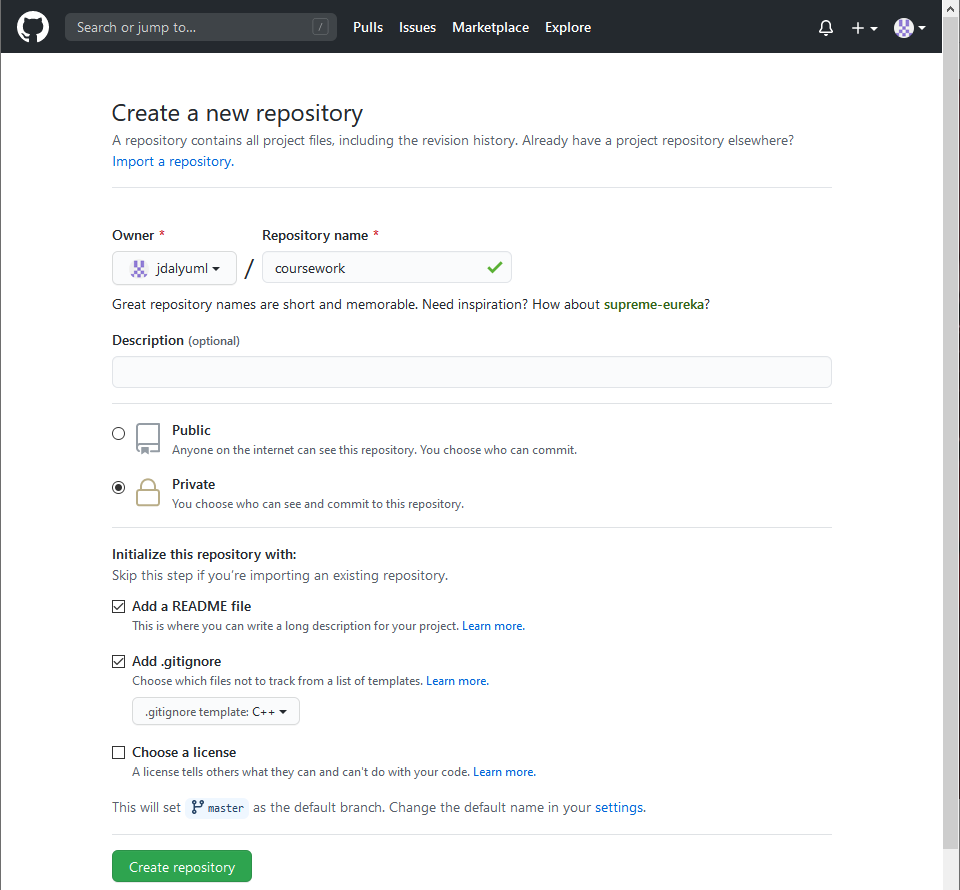
\includegraphics[width=0.7\columnwidth]{newrepo}

Once you have created your repository, go to the Settings tab, then select Manage Access and invite the instructor (\textbf{\instructor}) as a collaborator.
This will allow us access to the repository even though it is a private repository.
Once this assignment has been graded you can remove them as a collaborator.


\section{Clone the repository}

Now, we will clone the repository to your machine.
Open a terminal and navigate to the directory where you want to copy the repository.
On Windows, you can do this by opening the folder in Explorer, right clicking, and then selecting Git Bash from the context menu.

You can clone the repository using the command \code{git clone <repo url>} where \code{<repo url>} can be found on the Code tab of your GitHub repository by selecting the \textcolor{green}{green} download code button.

\section{Setup Directories}

Next, create a directory(folder) for one of your classes.
You can do this either in the terminal (by using the \texttt{mkdir} command) or with another program, such as Explorer.
It will be easier if you \textbf{don't} use spaces in the name.
A good name might be \texttt{computing1}.

Next, we will put the homework from your other class into this directory.
In a separate Explorer window, find the daily assignments from your Computing I course.
Copy the files and paste them into the \texttt{computing1} directory that you created.

You will now want to check that you have correctly copied the files over.
You can do this by typing \texttt{git status} into the terminal.
If you have done everything correctly so far, you should see the name of your directory in \textcolor{red}{red} text.
If you don't see it, type \texttt{ls} into the terminal to list the contents of the current directory.
If you don't see the directory, you probably mixed up your folders in Explorer.
If you do, type \texttt{ls <dirname>} to view all of the files in the directory.

\section{Stage your changes}

Creating files does not automatically add them to the repository.
We will add the new files to the ``staging area'', which contains file that are ready.
For each of the files, use \code{git add <filename>} to stage it.
If you put all of the files into a single directory, you can do this by adding that directory.
Once you have added all of the files, use \code{git status} to list all of the staged files (which will appear in \textcolor{green}{green}).
If you missed some, they will probably appear in \textcolor{red}{red}.

\section{Commit your changes}

Once all of your changes are staged, you will want to commit the changes.
You can use \code{git commit} to commit the changes.
This will open up an editor for you to type a message describing what changes you made.
Alternately, you can use \code{git commit -m ``<some message>''} (with parenthesis) to give a message directly to git without opening an editor.

The first time you do this, Git will tell you that you need to setup some information.
Use \code{git config --global user.name ``<username>''} to set your username and \code{git config --global user.email ``<email>''} to set your email.
Once you have done this, you won't have to do it again.
You can remove the \code{--global} to make this information apply only to this repository, but then you will have to enter it again for your next repository.

If you didn't change the editor back in Step \ref{sec:Install}, then Git may open the commit message in \href{https://www.vim.org/}{Vim}, a powerful editor, but one that takes time to get used to.
You can type \code{:qa} to close Vim and cancel your commit.
You can then use the Git installer to change the default editor or add the commit message as an argument.

\section{Push to GitHub}

Committing saves a local copy of all of your changes, but doesn't affect GitHub.
You can use \code{git push} to push your changes from your local machine up to GitHub.
You may be asked to supply your GitHub login credentials.
Once this is done, go to your repository on GitHub (or refresh the page) to verify that your changes have been posted.

\section{Submission}\label{sec:Submission}

Verify that your repository is marked private (this will appear at the top of your screen next to the repository name), that it contains a directory with some files in it, and that you have added the instructor (\textbf{\instructor}) as a collaborator.
Once you have done so, submit the URL of your repository on Blackboard.

\end{document}